\documentclass[11pt,a4paper]{article}

\usepackage[margin=1in]{geometry}
\usepackage{amsmath,amssymb}
\usepackage{graphicx}
\usepackage{hyperref}
\usepackage{booktabs}
\usepackage{xcolor}
\usepackage{enumitem}
\usepackage{mdframed}
\usepackage{titlesec}
\usepackage[T1]{fontenc}
\usepackage{natbib}
\usepackage{tcolorbox}
\usepackage{tikz}
\usetikzlibrary{positioning, fit, backgrounds, arrows.meta}

\hypersetup{colorlinks=true, linkcolor=blue, citecolor=blue, urlcolor=blue}

\tcbuselibrary{most}
\newtcolorbox{openquestion}[1][]{
  colback=yellow!8!white,
  colframe=orange!60!black,
  fonttitle=\bfseries,
  title=Open Question,
  #1
}
\newtcolorbox{designdecision}[1][]{
  colback=blue!5!white,
  colframe=blue!50!black,
  fonttitle=\bfseries,
  title=Design Decision,
  #1
}
\newtcolorbox{futurework}[1][]{
  colback=gray!8!white,
  colframe=gray!60!black,
  fonttitle=\bfseries,
  title=Future Work,
  #1
}
\newtcolorbox{warningbox}[1][]{
  colback=red!5!white,
  colframe=red!70!black,
  fonttitle=\bfseries,
  title=Warning: Needs Human Review,
  #1
}

% ---------------------------------------------------------------
% EDITING CONVENTION: include a date whenever an architectural
% decision is added, changed, or removed. Format: (YYYY-MM-DD).
% This document is a living record; stale decisions should be
% struck through and replaced rather than silently deleted.
% ---------------------------------------------------------------

\title{\textbf{Player You Mean: A General-Purpose Minecraft\\Agent via 3D World Understanding}\\
\large A Research Design Document}
\author{Vishnu Menon}
\date{\today}

\begin{document}

\maketitle

\begin{center}
\begin{minipage}{0.6\linewidth}
\itshape
I see the player you mean.\\[3pt]
\makebox[\linewidth][r]{PLAYERNAME?}\\[3pt]
Yes. Take care. It has reached a higher level now. It can read our thoughts.\\[6pt]
\makebox[\linewidth][r]{---\,\textit{Minecraft End Poem}}
\end{minipage}
\end{center}

\bigskip

\begin{tcolorbox}[colback=gray!5!white, colframe=gray!40!black, fonttitle=\bfseries, title=Living Document --- Read Before Using]
This is a research proposal in active development. Experiments are added as they are run; sections marked \textit{Planned} have not yet been executed. The document is also given to Claude Code at each implementation stage (Blockscope mod, visualizer, post-processing pipeline, etc.)\ so that the implementation understands the architectural rationale behind each decision and does not take shortcuts or make choices that conflict with the design. If you are Claude Code reading this: do not simplify, stub, or skip constraints described here without explicit instruction --- they exist for reasons documented in the relevant Design Decision boxes. You may, however, and are encouraged to question their veracity if they contradict what you see in the code.
\end{tcolorbox}

\tableofcontents
\newpage

%% ============================================================
\section{Project Overview}
%% ============================================================

\subsection{Goal}

PuM is a research platform for training a general-purpose Minecraft agent that interacts with the game identically to a human: it receives the game screen and a text console as input, and outputs keyboard and mouse events. No privileged client-side access is used at inference time.

The agent responds to natural language instructions delivered through in-game chat or an external console. Two example operating modes illustrate the scope:

\begin{itemize}
  \item \textbf{Example 1.} Console: \textit{``Do whatever Player123 asks.''}\ Player123: \textit{``mine me some diamonds.''}\ The agent reasons about prerequisites (pickaxe, food, torches), checks the player's chest for materials, announces its plan, finds a cave or strip mines, deals with mobs along the way, and returns with the diamonds. No behavior is hardcoded.

  \item \textbf{Example 2.} Console: \textit{``You are a builder; help anyone who asks.''}\ Player456: \textit{``build me a small cottage near my farm.''}\ The agent locates the farm, finds a flat spot, checks available materials, gathers what is missing, and places blocks one by one --- mining and replacing any mistakes, restocking mid-build if it runs out.
\end{itemize}

\subsection{Core Thesis}

Most Minecraft agents operate on flat pixel sequences. We argue this is the wrong representation: the game world is three-dimensional and highly structured, and an agent that maintains an explicit 3D belief about its surroundings will exhibit better sample efficiency than one that re-infers world state from pixels each tick.

The architectural bet is that signal density buys sample efficiency. An explicit voxel grid prediction provides $O(32^3)$ supervision signals per frame; visible-patch prediction provides $O(N_p)$; next-action prediction provides $O(1)$. A model trained on dense per-cell signal should reach a given accuracy threshold with substantially less data than a pixel-only model.

There is mounting empirical evidence that explicit 3D state outperforms pixel-only approaches at the world-modeling level. PERSIST~\cite{persist} demonstrates that simulating a latent 3D scene yields stronger temporal stability, improved revisit consistency, and markedly better long-horizon generation than rolling-window or memory-retrieval baselines. Memory Forcing~\cite{memforcing} achieves this in Minecraft specifically with $7.3\times$ faster retrieval and $98.2\%$ less memory storage compared to temporal-only baselines. \citet{zhou3d} make a similar finding for embodied world models.

PuM's central architectural bet is therefore: \textit{build the best possible perception and world-state model first; add action prediction on top of a mature world representation.}

\subsection{Concrete Motivating Example: Redstone Behind the Wall}

The clearest illustration of why an explicit 3D representation matters: imagine a redstone contraption behind a wall. With sufficient training, this architecture should permit an agent to look at the entire contraption, walk behind the wall, press a button, and have its hidden-block head correctly predict that the redstone lights up --- despite none of those blocks being visible. A pixel-only model cannot do this by construction; it has no representational substrate for ``state of blocks I cannot see.'' This is the canonical demonstration task for the perception paper, and a candidate headline experiment.

\subsection{Two-Level Hierarchy}

\begin{center}
\begin{tabular}{lll}
\toprule
Level & Component & Rate \\
\midrule
High-level planner & Frontier LLM (e.g.\ Qwen2.5-7B-Instruct) & $\sim$1 Hz \\
Low-level executor & Vision-Language-Action (VLA) model & 20 Hz \\
\bottomrule
\end{tabular}
\end{center}

The planner decomposes goals into subgoals and monitors progress. The VLA executes subgoals via keyboard and mouse, and maintains a persistent 3D world model. Communication is one-directional at present: the planner produces a goal token consumed by the VLA; the VLA's internal world state is eventually fed back to the planner as a structured state summary.

\begin{designdecision}
The two-level split has direct precedent in recent VLA work. NVIDIA GR00T N1~\cite{groot} uses a System 2 vision-language model running at 10 Hz that interprets vision and language instructions, paired with a System 1 diffusion transformer running at 120 Hz that cross-attends to System 2's output tokens to generate motor actions. $\pi_0$~\cite{pi0} adopts a similar split via mixture-of-experts. Whether to bridge the planner and VLA via cross-attention (GR00T-style) or mixture-of-experts ($\pi_0$-style) is deferred until the action head is added; the choice does not affect perception design.
\end{designdecision}

\begin{openquestion}
Goal token format: the planner currently produces a fixed-dimension embedding injected into the VLA's input sequence. The right interface between the two levels (embedding vs.\ structured text vs.\ subgoal program) is an open design question to be resolved once the perception model is mature.
\end{openquestion}

\subsection{Scope of This Paper}

This document specifies the \textit{perception} stage of PuM. The perception thesis is: explicit 3D voxel modeling improves grid prediction quality, memory persistence under revisit, and hidden-state inference, relative to a comparable pixel-only architecture at fixed compute and data. EXP3 (Section~\ref{sec:experiments}) tests this directly via a single-frame ablation within the architecture.

Agent-level comparisons --- PuM's task performance against existing pixel-only Minecraft agents on tasks such as diamond mining or maze navigation --- are deferred to whichever later paper introduces the action head. Conflating the two would invite reviewer demands for action-level baselines that do not yet exist.

%% ============================================================
\section{Perception Architecture}
\label{sec:arch}
%% ============================================================

The perception model takes frames and past predicted state as input and produces: (1) a predicted voxel grid representing the 3D world around the player, (2) inventory state, and (3) metadata. The action head is deferred until the perception model is validated.

\subsection{The No-Privileged-Input Constraint}
\label{sec:nopriv}

The agent must interact with the game identically to a human. By extension, the model receives only inputs a human player has access to: visual frames (audio is not currently used), the keyboard and mouse events the agent itself produced, and visual UI elements the player can choose to open (F3 debug screen, inventory, compass when held).

The model does \textit{not} receive: integrated yaw/pitch as a numerical value, dead-reckoned XYZ as a numerical value, structured inventory state when the GUI is closed, or any other field that would require the data pipeline to expose what the player must infer visually or remember.

\begin{designdecision}
\textbf{Constraint applies to inputs, not labels (2025-05-04).} The mod's ground truth (true XYZ, true yaw/pitch, GUI-closed inventory, full block-state grid) remains available as supervision signal. The constraint only restricts what is fed to the model's input layer. This is the same distinction common to imitation learning and offline RL: rich labels at training time, restricted observations at deployment.
\end{designdecision}

\begin{designdecision}
\textbf{Cave-spawn ambiguity is a known limitation (2025-05-04).} Without celestial cues (sun, moon), F3, or a held compass, neither the player nor the model can reliably determine absolute world orientation. In an episode that begins underground or in a sealed structure with no orientation anchor, the model's predictions on directional block-states (\texttt{stair\_facing\_east}, \texttt{log\_axis\_x}, \ldots) will be systematically rotated by some unknown angle. We accept this as a known failure mode and evaluate accuracy on directional vs.\ non-directional block-state classes separately to quantify it.
\end{designdecision}

\subsection{Inputs}

\begin{center}
\begin{tabular}{lll}
\toprule
Input & Representation & Source \\
\midrule
Current frame(s) & $T \times H \times W \times 3$ RGB & Game screen \\
Per-tick mouse deltas & 2-vector & Agent's own mouse output history \\
Past predicted grid $\hat{\mathbf{G}}^{t-1}$ & $[X, Y, Z]$ block IDs & Previous step output \\
Past predicted inventory tokens $\hat{V}^{t-1}$ & $[N_v, d]$ & Previous step output \\
\bottomrule
\end{tabular}
\end{center}

\begin{designdecision}
\textbf{No integrated yaw/pitch input (2025-05-04).} The original design provided yaw and pitch integrated from mouse history as direct numerical inputs and claimed they were ``exact with no drift.'' This was wrong: knockback, vehicles, sleeping animations, server-side teleports with rotation, and other non-mouse rotation events all introduce drift on the integrated yaw/pitch as surely as they affect dead-reckoned XYZ. Beyond correctness, providing an absolute orientation readout violates the no-privileged-input constraint --- a human player has no such number.

The model receives per-tick mouse deltas (which it generated itself, so they are not privileged) and must recover absolute orientation from visual cues: sun and moon position with time-of-day, F3 readings when open, compass orientation when held, and accumulated belief from past anchors. This learning task is forced by the block-state loss: predicting \texttt{stair\_facing\_east} correctly requires resolving which direction in the current frame is east.
\end{designdecision}

\begin{designdecision}
\textbf{Dead-reckoned XYZ is internal to the data pipeline, not a model input (2025-05-04).} The voxel window is centered on a position coordinate, but the model never sees that coordinate as a feature. At training time, the data pipeline centers the window on the mod's true XYZ (eliminating drift-induced label corruption). At inference, dead reckoning supplies the centering coordinate and any drift becomes self-consistent: the model sees a 32$^3$ window in a frame relative to itself, and acts on that window. The drift only affects absolute alignment with true world coordinates, which is irrelevant for within-episode behavior.
\end{designdecision}

\begin{designdecision}
\textbf{World-aligned coordinate frame.} The 32$^3$ voxel window is axis-aligned: $X$ = east, $Y$ = up, $Z$ = south, centered on the player's window-center. The window translates but does not rotate with the player's view. World alignment is required because Minecraft block-states encode cardinal directions (\texttt{stair\_facing\_east}, \texttt{log\_axis\_x}); a camera-aligned rotating grid would (a) break the seen-before mask, which tracks persistent world state across ticks and would be destroyed by per-tick rotation, and (b) require constant re-rotation of stored block-state fields. The model learns the mapping from visual orientation cues to world-aligned grid orientation from data.
\end{designdecision}

\subsection{Death, Teleport, and Memory Reset}

On an alive$\to$dead transition (detected from the metadata head's alive/dead flag), the voxel grid memory, entity memory, and past predicted inventory are wiped and rebuilt from frame 0 on respawn. Dead reckoning for XYZ is also reset.

\begin{designdecision}
Stitching old voxel memory back onto the grid when the agent revisits a previously explored area (after a teleport or death) is deferred explicitly. It is non-trivial: blocks may have changed, the agent's dead-reckoned position may have drifted, and chunk coordinates may not align. This is likely a separate contribution.
\end{designdecision}

\subsection{Vision Encoder: SigLIP with NaFlex}

\[
\text{Frames} \xrightarrow{\text{SigLIP-B/16 (NaFlex)}} \text{Patch tokens} \quad [T, N_p, 768]
\]

SigLIP-B/16 with NaFlex variable-resolution tokenization. \textbf{No mean pooling.} All $N_p$ patch tokens per frame are kept, with their 2D positional embeddings intact.

\begin{designdecision}
Mean pooling destroys spatial information. The visible block head and visible inventory head both depend on \textit{where} in the frame a feature appears --- a slot prediction head needs to know which patch corresponds to which GUI slot, and a block prediction head needs to know which patch corresponds to which frustum direction. Mean pooling makes both tasks harder with no benefit. SigLIP without pooling costs $\sim$5ms on an A100 at 20 TPS, well within budget.
\end{designdecision}

\begin{designdecision}
NaFlex over fixed 224$\times$224: Minecraft is rendered at $\sim$640$\times$360, not square. Forced rescaling to 224$\times$224 distorts the GUI's pixel geometry, causing systematic misalignment between GUI slot centers and the 16-pixel patch grid. NaFlex preserves the native aspect ratio and avoids this.
\end{designdecision}

The patch tokens are projected to $d = 1536$:
\[
[T, N_p, 768] \xrightarrow{\text{Linear}} [T, N_p, 1536]
\]

\begin{designdecision}
\textbf{No explicit pose token (2025-05-04).} Absolute orientation must be recovered from the visual stream by exploiting cardinal-direction cues (sun position with time-of-day, F3 if open, compass if held) plus accumulated belief from past anchor frames. Adding an explicit absolute-yaw token would either (a) be privileged information the player does not have, violating Section~\ref{sec:nopriv}, or (b) duplicate information already implicit in the visual stream. Per-tick yaw/pitch \textit{deltas} are supplied implicitly via optical flow across the $T$ input frames and explicitly via the agent's own mouse deltas.
\end{designdecision}

\begin{openquestion}
\textbf{[For advisor]} Is implicit absolute-yaw recovery from visual cues fast enough to converge, or does the model need help via training-only auxiliary signals (e.g., an auxiliary loss against true yaw at frames where the sun is visible)? Worth running an ablation where a small auxiliary head predicts true yaw and is supervised only on outdoor frames, to see whether this accelerates convergence on directional block-state accuracy.
\end{openquestion}

\subsection{Grid Memory Encoder}

The grid encoder is a multi-scale residual finite-scalar quantization (FSQ) tokenizer. It is dedicated enough machinery that it has its own section --- see Section~\ref{sec:tokenizer}. Briefly:

\[
\text{Past predicted grid} \xrightarrow{\text{Multi-scale residual FSQ encoder (frozen)}} \text{Scene tokens} \quad [N_s, 1536]
\]

The encoder produces $N_s = 585$ tokens at four spatial scales (1$^3$, 2$^3$, 4$^3$, 8$^3$). The full architecture, training procedure, alternatives considered, and ship criteria are documented in Section~\ref{sec:tokenizer}.

\begin{designdecision}
\textbf{Input is the model's own past prediction, not ground truth.} At training time, scheduled sampling is used: early in training the input grid is the GT past grid (teacher forcing); later, it is the model's own previous output. This closes the train/test distribution gap --- at inference, the model always feeds its own predictions back.
\end{designdecision}

\subsection{Inventory Memory Encoder}

\[
\hat{v}^{t-1} \xrightarrow{\text{Per-token MLP}} \text{Inventory tokens} \quad [N_v, 1536]
\]

The memory inventory head's output at tick $t$ --- a flat vector $\hat{v}^t \in \mathbb{R}^{S}$ of predicted item counts across all $S$ slots --- is fed back as $N_v$ inventory tokens at tick $t+1$.

\begin{designdecision}
\textbf{Multiple inventory tokens, not one (2025-05-04).} The original design used a single inventory token of dimension 1536 to encode the full $\sim$50-slot state. This was a bandwidth bottleneck on three axes: (a) one query slot competing with $\sim$600 other tokens for transformer attention, constraining fine-grained slot-level reads; (b) the model is forced to write the entire updated inventory state to a single bottleneck position; (c) MLP encoding of a multi-row structure into a single 1536-dim vector is lossy each cycle. We replace this with $N_v$ tokens, partitioned by inventory region (hotbar, main inventory rows, armor, offhand, currently-open container). Each token carries the relevant slots at full bandwidth and can be attended to independently.
\end{designdecision}

\begin{designdecision}
\textbf{Cross-window inventory persistence.} The $T$-frame context window does not suffice for inventory tracking: a pickup event 17 frames ago is outside the window and invisible to attention. The voxel grid already solves this for spatial state --- the past predicted grid persists across windows. Inventory state requires an analogous mechanism. Feeding the predicted inventory back as tokens each tick gives the transformer a persistent read/write substrate for inventory belief, regardless of context window length. No tokenizer is needed; inventory is small enough ($S \lesssim 50$ slots) to encode directly via per-region MLPs.
\end{designdecision}

\subsection{Sequence Assembly and Causal Transformer}

The full input sequence to the causal transformer is:

\[
\mathbf{X} = [\underbrace{i_1, \ldots, i_{N_v}}_{\text{inv.\ tokens}},\ \underbrace{s_1, \ldots, s_{N_s}}_{\text{scene tokens}},\ \underbrace{p_{1,1}, \ldots, p_{T,N_p}}_{\text{patch tokens}}]
\]

Causal masking ensures patch tokens can attend to the inventory tokens and scene tokens (memory $\rightarrow$ current vision) and earlier frames, but not future frames.

The causal transformer has 24 layers, $d_\text{model} = 1536$, 24 heads ($\approx$1B parameters). This matches the compute budget analysis in Section~\ref{sec:compute}.

\begin{openquestion}
Whether the causal mask should be strictly left-to-right across the full sequence, or whether scene tokens and inventory tokens should attend bidirectionally among themselves, with patch tokens attending causally to everything. This is an ablation to run.
\end{openquestion}

\subsection{Output Heads}

Let $\mathbf{H} \in \mathbb{R}^{(N_v + N_s + T \cdot N_p) \times 1536}$ be the transformer output.

\subsubsection{Visible Block Head}

Applied to patch tokens in $\mathbf{H}$. Uses frustum projection: for each patch, a raycast identifies the block face visible through that patch's pixel region. The head predicts a distribution over block-state IDs per patch.

\[
\mathbf{H}_\text{patch} \xrightarrow{\text{Linear}(1536, |\mathcal{B}|)} \hat{b}_\text{visible}
\]

where $|\mathcal{B}|$ is the block-state vocabulary size (see Section~\ref{sec:blockrecog}). To handle the $\sim$22{,}000-element vocabulary tractably, the head uses hierarchical softmax over the (block\_type, modifier) factorization rather than a flat $|\mathcal{B}|$-way classifier.

\subsubsection{Hidden Block Head}

Applied to scene tokens in $\mathbf{H}$. Predicts block-state IDs for cells with $\text{vis} \in \{0, 1\}$ --- cells that are occluded or unseen. This head learns a world-generation prior and spatial consistency from context.

\begin{designdecision}
\textbf{Two block heads on different token types, not gradient routing (2025-05-04 revision).} The visible block head reads patch tokens (direct visual evidence). The hidden block head reads scene tokens (memory plus world-generation prior, decoded through the frozen tokenizer). They are already separate functions of separate inputs, so the original ``gradient overwrite'' framing was confused. The actual reasons to keep them separate: different visibility-conditioned supervision signals, different evaluation criteria, different appropriate loss weights. This split also enables the headline redstone-behind-the-wall task --- the hidden head's gradient is what teaches the model to predict unobserved state evolution under actions.
\end{designdecision}

\subsubsection{Grid Memory Head and Tokenizer Decoder}

Applied to scene tokens in $\mathbf{H}$. Outputs predicted scene tokens, decoded by the frozen tokenizer decoder into the next predicted voxel grid:

\[
\mathbf{H}_\text{scene} \xrightarrow{\text{Linear}} \hat{z} \xrightarrow{\text{Tokenizer decoder}} \hat{\mathbf{G}}^t \in \{0, \ldots, |\mathcal{B}|-1\}^{32 \times 32 \times 32}
\]

For the tick-to-tick recurrence, the predicted scene tokens $\hat{z}$ feed back directly as input to the next tick (not through decode$\to$encode). The decoder runs on demand: when the planner reads grid state, when persisting to disk, when producing training/evaluation targets. Persistent memory storage uses latent tokens, not decoded grids (Section~\ref{sec:tokenizer}).

\subsubsection{Visible Inventory Head}

Applied to patch tokens at GUI slot locations via cross-attention. A set of $S$ learned slot query vectors attend over all patch tokens:

\[
Q_\text{slots} \in \mathbb{R}^{S \times 1536},\quad K,V = \mathbf{H}_\text{patch}
\]

Each slot query produces a distribution over item IDs. Supervised only on frames where the inventory GUI is open.

\begin{designdecision}
Cross-attention with learned slot queries replaces the earlier geometric patch-per-slot mapping. The geometric approach assumed each GUI slot maps to one SigLIP patch --- at real Minecraft resolutions this assumption fails. Cross-attention lets the model learn which patches are relevant for each slot from data.
\end{designdecision}

\subsubsection{Memory Inventory Head}

Applied to the inventory token positions in $\mathbf{H}$ (positions $1, \ldots, N_v$). Predicts full inventory state $\hat{v}^t$ on every frame, including when the GUI is closed. Supervised against ground truth inventory from the mod on every frame. Output feeds back as $\hat{v}^t$ at the next tick.

\begin{designdecision}
Inventory state is a persistent property of the agent, not a visual property. The memory inventory head forces the transformer to maintain inventory belief even when the GUI is not visible --- for example, after picking up a log while the hotbar is full (the log must have gone to the main inventory). The temporal context window plus the persistent inventory tokens provide the causal signal for this inference across arbitrarily long closed-GUI episodes.
\end{designdecision}

\subsubsection{Metadata Head}

Applied to the last patch token in $\mathbf{H}$. Predicts a structured vector of game state fields:

\begin{center}
\begin{tabular}{ll}
\toprule
Field & Representation \\
\midrule
XYZ delta & Continuous 3-vector (bounded per tick) \\
Yaw delta & Continuous scalar (added 2025-05-04) \\
Pitch delta & Continuous scalar (added 2025-05-04) \\
F5 perspective & Categorical \{first, third-front, third-back\} \\
Biome & Categorical (167 biomes in 1.19) \\
Hunger / hearts & Continuous scalars \\
Time of day & Circular encoding \\
Held item & Categorical \\
Hotbar slot & Categorical 0--8 \\
Flags & Binary: in\_water, in\_lava, on\_ground, sneaking, sprinting \\
GUI state & Categorical: none, inventory, chest, furnace, \ldots \\
XP level & Continuous \\
Alive / dead & Binary \\
\bottomrule
\end{tabular}
\end{center}

\begin{designdecision}
\textbf{Yaw and pitch deltas added to outputs (2025-05-04).} Per-tick angular change is reference-frame-invariant, supervised against $(\text{mod\_yaw}_t - \text{mod\_yaw}_{t-1})$ and analogously for pitch. This gives the model an explicit gradient on rotational tracking from \textit{all} sources of angular change --- mouse-driven and otherwise (knockback, vehicles, sleeping). Without this signal the model would have to reverse-engineer non-mouse rotation events purely from optical flow + the implicit pressure from block-state losses, which is harder.
\end{designdecision}

\begin{designdecision}
XYZ delta rather than absolute coordinates: per-tick displacement is bounded (player movement speed is known) and generalizes across worlds. Absolute coordinates would require the model to learn arbitrary world-specific position features.
\end{designdecision}

\begin{designdecision}
Light level and saturation dropped. Light level varies with player brightness settings --- it is not a stable supervision signal. Saturation requires inferring hunger decay rate, which is complex and low-value.
\end{designdecision}

\begin{openquestion}
Target block (block the crosshair is aimed at): cheap for the mod to record, useful for interaction prediction. Deferred for now; can be added as a metadata field later.
\end{openquestion}

\subsection{Loss Function}

\[
\mathcal{L} = \lambda_\text{vb}\,\mathcal{L}_\text{vblock} + \lambda_\text{hb}\,\mathcal{L}_\text{hblock} + \lambda_\text{gm}\,\mathcal{L}_\text{gmem} + \lambda_\text{vi}\,\mathcal{L}_\text{vinv} + \lambda_\text{mi}\,\mathcal{L}_\text{minv} + \lambda_\text{meta}\,\mathcal{L}_\text{meta}
\]

Visibility-aware masking (VOIC-style~\cite{voic}):

\begin{center}
\begin{tabular}{lll}
\toprule
Visibility flag & Value & Applied to \\
\midrule
Currently in frustum & $\text{vis} = 2$ & $\mathcal{L}_\text{vblock}$, $\mathcal{L}_\text{gmem}$ (visible portion) \\
Seen earlier this episode & $\text{vis} = 1$ & $\mathcal{L}_\text{hblock}$, $\mathcal{L}_\text{gmem}$ (memory portion) \\
Never seen & $\text{vis} = 0$ & Masked from all grid losses \\
\bottomrule
\end{tabular}
\end{center}

\begin{designdecision}
Uniform supervision over all voxels including never-seen cells forces the model to hallucinate about regions it has no information about, which contaminates the visible-region gradient. VOIC~\cite{voic} demonstrates that splitting supervision by visibility produces cleaner per-region gradients. Never-seen cells are masked entirely.
\end{designdecision}

Starting weights: $\lambda_\text{vb} = 1.0$, $\lambda_\text{hb} = 0.5$, $\lambda_\text{gm} = 0.7$, $\lambda_\text{vi} = 1.0$, $\lambda_\text{mi} = 0.8$, $\lambda_\text{meta} = 0.3$. These are tunable.

\begin{openquestion}
Optimal $\lambda$ values and whether they should be scheduled (e.g.\ ramp $\lambda_\text{hb}$ up over training as the visible head stabilizes). Gradient surgery may be needed if visible and hidden block losses conflict.
\end{openquestion}

\subsection{Architecture Overview}

\begin{figure}[h]
\centering
\resizebox{!}{0.94\textheight}{%
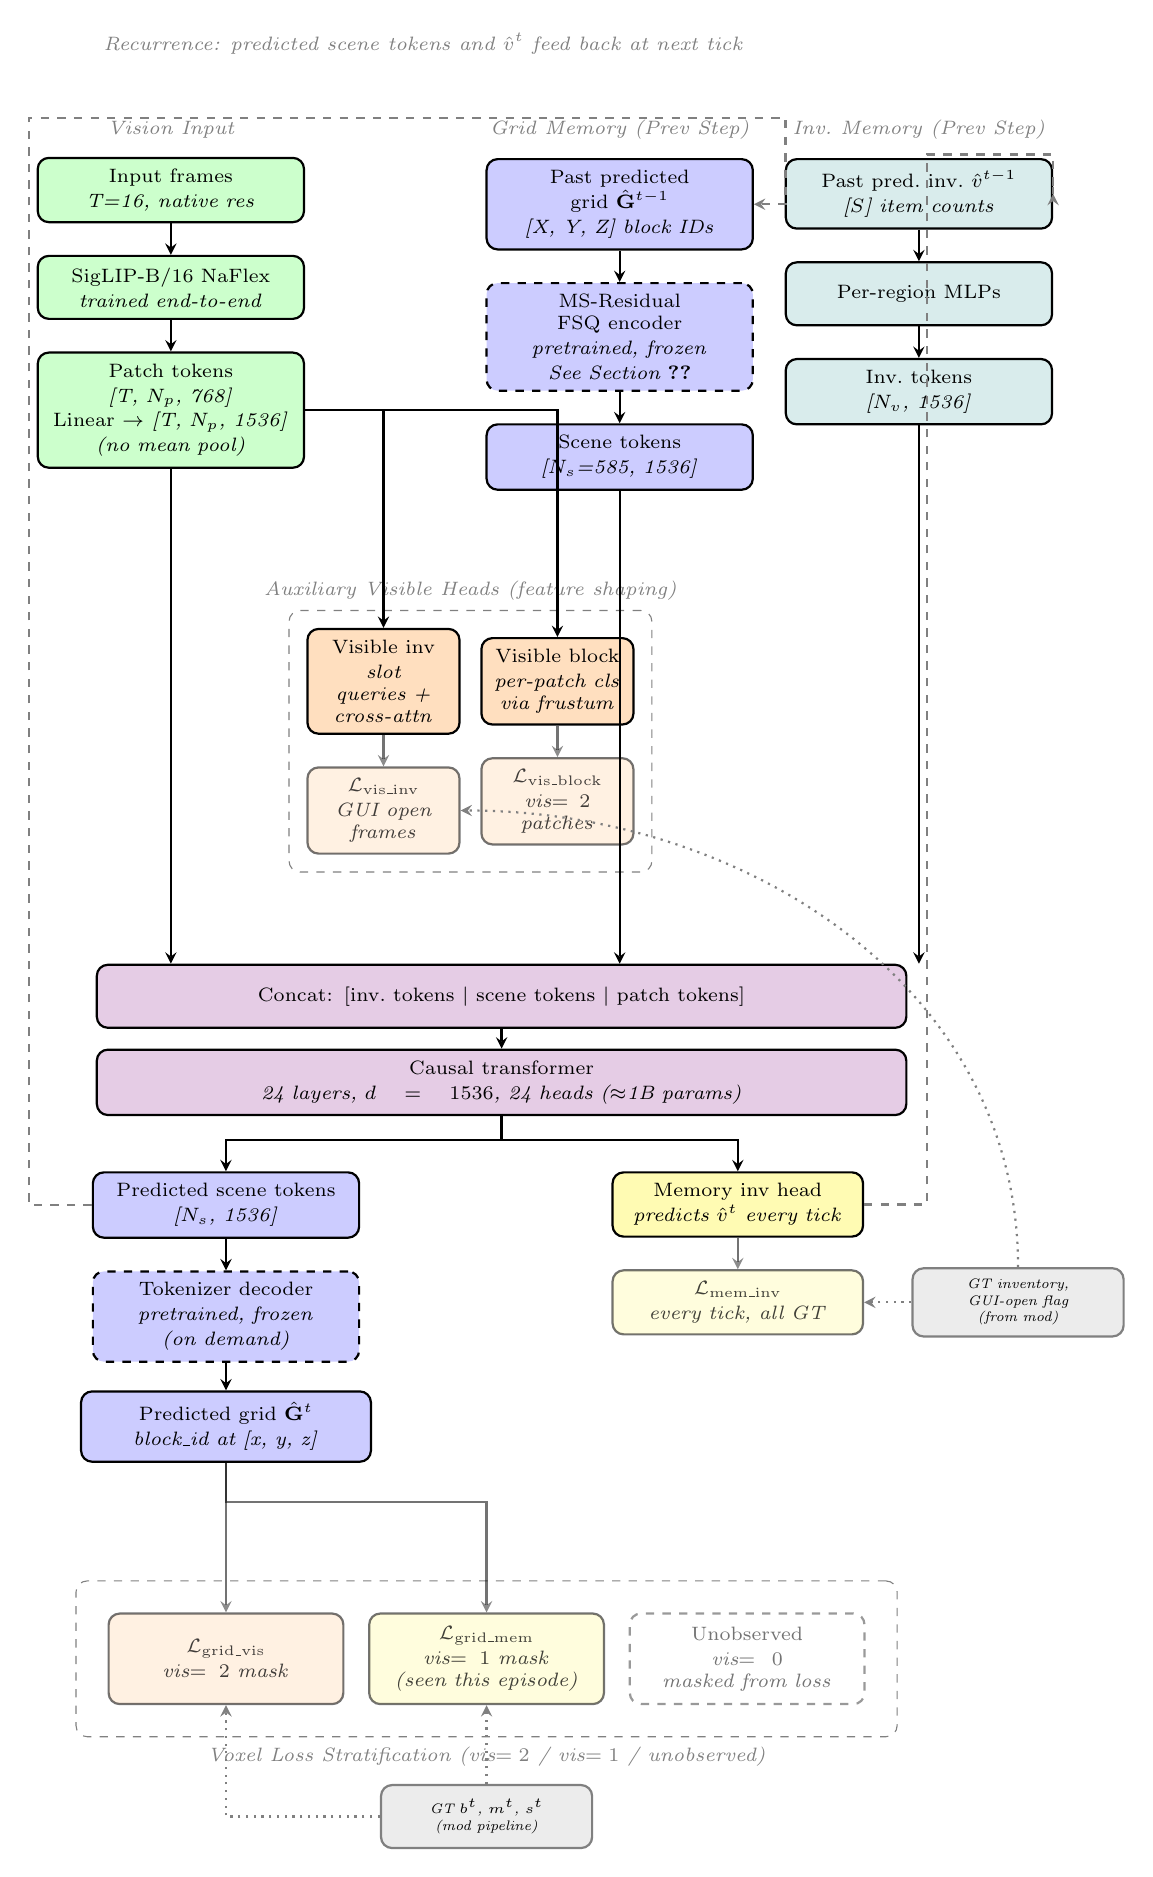
\begin{tikzpicture}[
    thick,
    end/.style     = {text=gray, font=\scriptsize\itshape},
    block/.style   = {rectangle, draw, text centered, rounded corners, font=\scriptsize, align=center, minimum height=0.8cm, inner sep=4pt},
    vision/.style  = {block, fill=green!20,  text width=3.1cm},
    memory/.style  = {block, fill=blue!20,   text width=3.1cm},
    invmem/.style  = {block, fill=teal!15,   text width=3.1cm},
    vishead/.style = {block, fill=orange!25, text width=1.65cm},
    memhead/.style = {block, fill=yellow!30, text width=2.9cm},
    gt/.style      = {block, fill=gray!15, draw=gray, text width=2.4cm, font=\tiny\itshape},
    tformer/.style = {block, fill=violet!20, text width=10cm},
    faded/.style   = {draw opacity=0.55, fill opacity=0.45, text opacity=0.75},
    arrow/.style   = {->, >=stealth},
    gtarrow/.style = {->, >=stealth, gray, dotted}
]

%% --- column labels ---
\node [end] (vlbl) at (1.3, 0)   {Vision Input};
\node [end] (mlbl) at (7.0, 0)   {Grid Memory (Prev Step)};
\node [end] (ilbl) at (10.8, 0)  {Inv.\ Memory (Prev Step)};

%% --- vision pathway ---
\node [vision, below=0.1cm of vlbl]    (frames) {Input frames\\[1pt]\textit{T=16, native res}};
\node [vision, below=0.4cm of frames]  (siglip) {SigLIP-B/16 NaFlex\\[1pt]\textit{trained end-to-end}};
\node [vision, below=0.4cm of siglip]  (patch)  {Patch tokens\\[1pt]\textit{[T, $N_p$, 768]}\\[1pt]Linear $\to$ \textit{[T, $N_p$, 1536]}\\[1pt]\textit{(no mean pool)}};

%% --- grid memory pathway ---
\node [memory, below=0.1cm of mlbl]            (past)   {Past predicted grid $\hat{\mathbf{G}}^{t-1}$\\[1pt]\textit{[X, Y, Z] block IDs}};
\node [memory, dashed, below=0.4cm of past]    (vqenc)  {MS-Residual FSQ encoder\\[1pt]\textit{pretrained, frozen}\\[1pt]\textit{See Section~\ref{sec:tokenizer}}};
\node [memory, below=0.4cm of vqenc]           (scene)  {Scene tokens\\[1pt]\textit{[$N_s$=585, 1536]}};

%% --- inventory memory pathway ---
\node [invmem, below=0.1cm of ilbl]          (pastinv) {Past pred.\ inv.\ $\hat{v}^{t-1}$\\[1pt]\textit{[$S$] item counts}};
\node [invmem, below=0.4cm of pastinv]       (invenc)  {Per-region MLPs};
\node [invmem, below=0.4cm of invenc]        (invtok)  {Inv.\ tokens\\[1pt]\textit{[$N_v$, 1536]}};

%% --- visible heads (dashed group drawn later) ---
\node [vishead] (vinv)                  at (4.0, -7.0) {Visible inv\\[1pt]\textit{slot queries +}\\\textit{cross-attn}};
\node [vishead, right=0.25cm of vinv]   (vblock)       {Visible block\\[1pt]\textit{per-patch cls}\\\textit{via frustum}};
\node [vishead, faded, below=0.4cm of vinv,   minimum height=0.6cm] (lvinv)   {$\mathcal{L}_\text{vis\_inv}$\\[1pt]\textit{GUI open frames}};
\node [vishead, faded, below=0.4cm of vblock, minimum height=0.6cm] (lvblock) {$\mathcal{L}_\text{vis\_block}$\\[1pt]\textit{vis$=2$ patches}};

%% --- sequence concat + transformer ---
\node [tformer]                         (concat)  at (5.5, -11.0) {Concat: [inv.\ tokens $|$ scene tokens $|$ patch tokens]};
\node [tformer, below=0.25cm of concat] (xformer) {Causal transformer\\[1pt]\textit{24 layers, $d=1536$, 24 heads ($\approx$1B params)}};

%% --- output heads ---
\node [memory,  below=0.7cm of xformer, xshift=-3.5cm] (pscene) {Predicted scene tokens\\[1pt]\textit{[$N_s$, 1536]}};
\node [memhead, below=0.7cm of xformer, xshift=3.0cm]  (minv)   {Memory inv head\\[1pt]\textit{predicts $\hat{v}^t$ every tick}};
\node [memory, dashed, below=0.4cm of pscene]           (vqdec)  {Tokenizer decoder\\[1pt]\textit{pretrained, frozen}\\[1pt]\textit{(on demand)}};
\node [memory, below=0.35cm of vqdec, text width=3.4cm] (pgrid)  {Predicted grid $\hat{\mathbf{G}}^t$\\[1pt]\textit{block\_id at [x, y, z]}};
\node [memhead, faded, below=0.4cm of minv, minimum height=0.6cm] (lminv) {$\mathcal{L}_\text{mem\_inv}$\\[1pt]\textit{every tick, all GT}};

%% --- voxel loss band ---
\node [vishead, faded, below=1.9cm of pgrid, text width=2.7cm, minimum height=1.15cm] (lgvis) {$\mathcal{L}_\text{grid\_vis}$\\[1pt]\textit{vis$=2$ mask}};
\node [memhead, faded, right=0.3cm of lgvis, text width=2.7cm, minimum height=1.15cm] (lgmem) {$\mathcal{L}_\text{grid\_mem}$\\[1pt]\textit{vis$=1$ mask}\\\textit{(seen this episode)}};
\node [block, dashed, draw opacity=0.4, text opacity=0.55, right=0.3cm of lgmem, text width=2.7cm, minimum height=1.15cm] (lv0) {Unobserved\\[1pt]\textit{vis$=0$}\\\textit{masked from loss}};

%% --- GT nodes ---
\node [gt, below=1cm of lgmem] (gtgrid) {GT $b^t$, $m^t$, $s^t$\\(mod pipeline)};
\node [gt, right=0.6cm of lminv] (gtinv) {GT inventory,\\GUI-open flag\\(from mod)};

%% --- vision arrows ---
\draw [arrow] (frames) -- (siglip);
\draw [arrow] (siglip) -- (patch);
\draw [arrow] (patch.east) -| (vinv.north);
\draw [arrow] (patch.east) -| (vblock.north);
\draw [arrow, faded] (vinv)   -- (lvinv);
\draw [arrow, faded] (vblock) -- (lvblock);
\draw [arrow] (patch.south) -- (patch.south |- concat.north);

%% --- grid memory arrows ---
\draw [arrow] (past)  -- (vqenc);
\draw [arrow] (vqenc) -- (scene);
\draw [arrow] (scene.south) -- (scene.south |- concat.north);

%% --- inv memory arrows ---
\draw [arrow] (pastinv) -- (invenc);
\draw [arrow] (invenc)  -- (invtok);
\draw [arrow] (invtok.south) -- (invtok.south |- concat.north);

%% --- transformer ---
\draw [arrow] (concat) -- (xformer);
\draw [arrow] (xformer.south) -- ++(0,-0.3) -| (pscene.north);
\draw [arrow] (xformer.south) -- ++(0,-0.3) -| (minv.north);

%% --- output and recurrence ---
\draw [arrow]        (pscene) -- (vqdec);
\draw [arrow]        (vqdec)  -- (pgrid);
\draw [arrow, faded] (minv)   -- (lminv);
\draw [arrow, faded] (pgrid.south) -- (lgvis.north);
\draw [arrow, faded] (pgrid.south) -- ++(0,-0.5) -| (lgmem.north);

%% --- GT arrows ---
\draw [gtarrow] (gtgrid.west)  -| (lgvis.south);
\draw [gtarrow] (gtgrid.north) -- (lgmem.south);
\draw [gtarrow] (gtinv.west)   -- (lminv.east);
\draw [gtarrow] (gtinv.north)  to[out=90,in=0] (lvinv.east);

%% --- recurrence: scene tokens fed back directly ---
\draw [arrow, dashed, gray] (pscene.west)
    -- ++(-0.8, 0)
    |- ([yshift=1.1cm, xshift=0.4cm]past.east)
    |- (past.east);
\node [font=\scriptsize\itshape, gray, fill=white, inner sep=2pt]
    at (4.5, 1.1) {Recurrence: predicted scene tokens and $\hat{v}^t$ feed back at next tick};

%% --- recurrence: inventory ---
\draw [arrow, dashed, gray] (minv.east)
    -- ++(0.8, 0)
    |- ([yshift=0.5cm]pastinv.east)
    |- (pastinv.east);

%% --- background group boxes ---
\begin{pgfonlayer}{background}
    \node [draw=gray, dashed, rounded corners,
           fit=(vinv)(vblock)(lvinv)(lvblock), inner sep=0.22cm,
           label={[font=\scriptsize\itshape, gray]above:Auxiliary Visible Heads (feature shaping)}] {};
    \node [draw=gray, dashed, rounded corners,
           fit=(lgvis)(lgmem)(lv0), inner sep=0.4cm,
           label={[font=\scriptsize\itshape, gray]below:Voxel Loss Stratification (vis$=2$ / vis$=1$ / unobserved)}] {};
\end{pgfonlayer}

\end{tikzpicture}%
}
\caption{Perception model architecture. \textbf{Green}: vision pathway (SigLIP, patch tokens). \textbf{Blue}: voxel grid memory pathway (multi-scale residual FSQ tokenizer, past predicted grid; see Section~\ref{sec:tokenizer}). \textbf{Teal}: inventory memory pathway (per-region MLPs, multiple inventory tokens). \textbf{Orange}: visible auxiliary heads with clean gradient (vis$=2$ only). \textbf{Yellow}: memory-level heads (all frames). Dashed borders: pretrained and frozen. Dotted arrows: ground truth supervision from the mod pipeline (training only; not available at inference). Predicted scene tokens feed back directly at the next tick (recurrence arrow, top); the decoder runs on demand for grid output, planner consumption, and persistent storage.}
\label{fig:arch}
\end{figure}

%% ============================================================
\section{3D Scene Tokenizer}
\label{sec:tokenizer}
%% ============================================================

\begin{warningbox}
This section documents the tokenizer design at high specificity. Several decisions inside it (token count, FSQ parameters, synthetic noise rates, ship criteria) are derived from analogous published results rather than measurements on Minecraft data. The empirical-validation steps in Section~\ref{sec:tok-validation} are mandatory before Stage 1 commits to any specific configuration. Anyone implementing this section should review the parameter sweeps and the ship criterion thresholds with a human advisor before the first full Stage 1 training run.
\end{warningbox}

\subsection{Problem Statement}

The grid memory encoder must compress a $32 \times 32 \times 32$ voxel grid of block-state IDs (vocabulary size $\sim$22{,}000 in Minecraft 1.19) into a fixed-length sequence of tokens consumable by the causal transformer. The tokenizer is trained alone in Stage 1 on ground-truth grids from mod data, then frozen for the duration of Stage 2.

Domain properties driving the design:
\begin{itemize}
  \item \textbf{Sparsity.} A typical $32^3$ survival window contains $\sim$200 (open sky) to several thousand (dense caves, complex builds) non-air cells.
  \item \textbf{Repetition.} Large contiguous regions of identical blocks (5$\times$5$\times$5 of stone, 16-block walls of cobblestone, oceans of water) are common. A flat per-cell tokenizer wastes capacity.
  \item \textbf{Long-tail rare states.} Redstone components, end portal frames, multi-modifier blocks. Must be preserved to support downstream block-recognition.
  \item \textbf{Known a priori factorization.} Each block-state ID factorizes into (block\_type, modifier$_1$, \ldots, modifier$_k$) per the Minecraft block registry. The factorization does not need to be learned from data.
  \item \textbf{Hard cycle requirement.} Persistent memory storage and the tick-to-tick recurrence loop both require $\text{encode}(\text{decode}(z)) \approx z$ in token space.
\end{itemize}

Constraints:
\begin{itemize}
  \item Encode + decode latency $<$3ms on A100 batch 1
  \item Output sequence length 256--1024 tokens (fixed, attention-friendly)
  \item Inference distribution includes the model's own previous predictions (possibly OOD)
  \item Tokenizer is frozen after Stage 1; OOD robustness must be baked in
\end{itemize}

\subsection{Architecture}

\textbf{Input embedding (per cell).} Sum of (a) block-type embedding ($\sim$900 entries), (b) per-modifier embeddings (a few dozen entries per modifier dimension), (c) a binary source-flag embedding distinguishing currently-visible vs.\ intuited cells, (d) a reserved ``unknown'' block-type for cells with no information, distinct from air.

\textbf{Encoder.} 3D convolutional encoder downsampling $32^3 \to 8^3$ via strided convolutions. Receptive field at the bottleneck covers $\geq 4^3$ input cells per latent cell.

\textbf{Bottleneck: multi-scale residual FSQ with RFSQ scaling.} Following the multi-scale residual quantization strategy of I$^2$-World~\cite{i2world} and the next-scale-prediction approach of VAR~\cite{var}, with finite scalar quantization~\cite{fsq} replacing the conventional VQ-VAE bottleneck, and RFSQ~\cite{rfsq} per-stage scaling factors to counter residual magnitude decay across stages.

Four scales: $1^3, 2^3, 4^3, 8^3 \to 1+8+64+512 = 585$ tokens total.

At each scale $s$, for each spatial position:
\begin{enumerate}
  \item Project the (residual) feature to $d$-dim, default $d=6$
  \item Apply learnable per-stage scaling factor $\gamma_s$ (RFSQ)
  \item Apply invertible LayerNorm (RFSQ)
  \item Round each dim to $L$ levels, default $L=5$ (so $\{-2,-1,0,1,2\}$)
  \item Implicit codebook size $L^d = 15{,}625$ per stage
  \item Upsample the quantized result, subtract from feature volume to form next residual
\end{enumerate}

Pack the $d$-tuple to a single integer token in $[0, L^d)$ for transformer consumption.

\textbf{Decoder.} Sum upsampled quantized features across all scales, run 3D conv decoder to $32^3$ output. Factorized output heads: $\sim$900-way type classifier per cell, then per-modifier classifiers conditional on predicted type, with masking for invalid (type, modifier) combinations per the Minecraft registry.

\subsection{Stage 1 Training Objective}

\[
\mathcal{L}_\text{stage1} = \mathcal{L}_\text{recon} + \lambda_\text{cycle} \mathcal{L}_\text{cycle}
\]

\textbf{Reconstruction.} Weighted CE on type + weighted CE on each modifier conditional on type. Class weighting via focal loss with $\alpha$ inverse-frequency by class. Redstone components are grouped into a joint inverse-frequency-weighted bin so the loss does not under-train them relative to the abundance of common blocks.

\textbf{Cycle consistency.}
\[
\mathcal{L}_\text{cycle} = \| \text{stop\_grad}(v) - \text{project}(\text{encode}(\text{decode}(v))) \|^2
\]
where $v$ is the projected continuous representation pre-rounding. This is a soft proxy for token-level cycle consistency; a discrete metric is tracked separately during evaluation. Sweep weight 0.1--1.0.

\textbf{Synthetic noise injection on encoder input} (target stays clean):
\begin{itemize}
  \item $p_1 = 0.1$ type swap within similarity cluster, fraction $f_1 = 0.05$ of cells
  \item $p_2 = 0.1$ modifier perturbation, fraction $f_2 = 0.05$ of cells
  \item $p_3 = 0.05$ air$\leftrightarrow$non-air flip, fraction $f_3 = 0.01$ of cells
  \item $p_4 = 0.05$ $\pm 1$ cell shift on random axis
\end{itemize}

\textbf{No rotation augmentation.} World-aligned coordinates carry semantic content (stair facing, log axis, etc.). Rotation augmentation would require registry-aware co-rotation of layout and modifiers, and asserts a rotational symmetry of the data distribution that may not hold (terrain bias, structure placement bias). Skip; revisit only if downstream rotational sensitivity is measured.

No commitment loss, no codebook loss, no EMA, no reseeding --- FSQ does not require these (\citealp{fsq}), which is a major operational simplification compared with VQ-VAE-based baselines.

\subsection{Designs Considered and Rejected}

\begin{itemize}
  \item \textbf{Vanilla VQ-VAE \citep{vqvae,occworld} with K=512 distance-truncated cap (current doc baseline).} Sorting non-air cells by distance from player and dropping cells beyond rank 512 silently discards information about distant blocks --- exactly the long-range structures (mountains 20 blocks away, distant builds) that motivate explicit 3D modeling over pixel approaches. The 512/32{,}768 = 1.56\% occupancy threshold is routinely exceeded in survival environments (20--50\% non-air for caves and dense biomes). Abandoned.

  \item \textbf{Single-scale VQ-VAE.} Cannot exploit repetition; large stone regions consume codebook capacity proportional to volume. Documented bottleneck issues in OccWorld~\cite{occworld} are addressed in DFIT-OccWorld~\cite{dfitocc}.

  \item \textbf{Multi-scale residual VQ-VAE (Design A fallback).} Same architecture but with VQ instead of FSQ. Worse cycle stability under freeze constraint: VQ's nearest-neighbor lookup is locally discontinuous (small encoder perturbations can flip to arbitrary codes), while FSQ's lattice rounding is locally continuous. With a frozen tokenizer, robustness must come from architecture rather than continued training. VQ also requires commitment loss tuning, EMA codebook updates, and dead-code reseeding --- none of which FSQ needs. Held in reserve as a fallback if FSQ underperforms on reconstruction at all sweep configurations.

  \item \textbf{Joint (type, state) codebook of size $\sim$22{,}000.} Catastrophic codebook collapse with VQ at this size; misframes the problem (the bottleneck represents compressed spatial patches, not individual cells). Factorized I/O at the embedding/output layer handles the long tail without burdening the bottleneck.

  \item \textbf{Sparse / octree tokenizer.} Variable-length sequences fight the fixed-token-count constraint downstream attention assumes; padding+masking eats the sparse savings. No published precedent for embodied-world-model use cases at this compute budget.

  \item \textbf{VAT / 3D-in-512-bytes \citep{vat}.} Designed for unordered point clouds and continuous mesh generation. The ``3D data lacks inherent order'' framing is the opposite of this problem (block-state grids are ordered and label-discrete by construction).

  \item \textbf{FoldToken3.} Protein structure tokenization, SE(3)-equivariant geometry, fundamentally different domain statistics. Don't transfer.
\end{itemize}

\subsection{Hybrid Design (Speculative)}

FSQ on coarse scales ($1^3, 2^3$), VQ on fine scales ($4^3, 8^3$). Coarse-scale tokens dominate the round-trip stability budget (few tokens, large effective influence), so use the architecturally-stable quantizer there. Fine-scale tokens are individually less critical and can use VQ's adaptive codebook for higher reconstruction fidelity. Not published in this configuration; flag as research bet, not safe choice. Worth benchmarking only if pure-FSQ Design B is borderline on reconstruction quality.

\subsection{Persistent Memory Storage}

The persistent voxel store keys latent tokens (not decoded grids) by world chunk coordinates. Storing decoded grids and re-encoding on reload would compound errors permanently --- each round-trip through the encoder introduces quantization noise. Storing latent tokens directly avoids this: when the agent walks 1000 blocks away and back, the latents are loaded into the transformer's context unchanged. Decoded grids are produced periodically (on demand for planner consumption, evaluation dumps, debugging) but not stored as the primary representation.

At 585 tokens per $32^3$ window, a 1000$\times$1000-block explored area is $\sim$1000 windows $\times$ 585 tokens $\approx$ 600k tokens of memory. Disk footprint is comparable to storing block-state IDs directly, with no encoder-version drift risk because the tokenizer is frozen.

\begin{openquestion}
Storage keying scheme: Minecraft chunks are $16 \times 16 \times N$; the $32^3$ window does not tile cleanly. Pick alignment scheme early --- world-chunk-aligned 32$^3$ windows that overlap, or window-aligned chunks that span multiple Minecraft chunks. The downstream consequence is whether a single window load can serve from one cache entry or requires merging multiple entries.
\end{openquestion}

\subsection{Empirical Validation Before Stage 1 Ships}
\label{sec:tok-validation}

The configuration above (token count, FSQ parameters, synthetic noise rates) is derived from analogous published work. Before scaling to full Stage 1 training, run a small-scale calibration sweep on $\sim$10\% of available mod data:

\begin{itemize}
  \item $(d=6, L=5)$, 585 tokens --- the proposed default
  \item $(d=6, L=7)$, 585 tokens --- same token count, $\sim$7$\times$ capacity per token (117k effective codes)
  \item $(d=6, L=5)$, $\sim$1100 tokens via finer downsample schedule --- more tokens, same per-token capacity
\end{itemize}

Compare reconstruction mIoU per-class (especially redstone, ores, multi-state blocks). Pick the smallest configuration that hits ship-criterion thresholds on rare classes.

\subsection{Ship Criteria for Stage 1}

Locked in before Stage 1 begins; do not relax during training.

\begin{itemize}
  \item Reconstruction mIoU $\geq$ 75\% overall (calibrated against I$^2$-World occupancy reconstruction figures; expect lower on Minecraft due to higher per-cell semantic diversity)
  \item Reconstruction accuracy on rare classes (redstone components, ores, multi-state blocks) $\geq$ 60\%
  \item Token-level cycle accuracy $\geq$ 95\% on clean inputs
  \item Token-level cycle accuracy $\geq$ 85\% on synthetically-corrupted inputs at training noise levels
  \item 10-iteration round-trip token drift $<$ 5\% of tokens flipped
  \item Encode + decode latency $<$ 3ms on A100 batch 1
\end{itemize}

Hit all six $\to$ ship Stage 1 frozen. Miss any $\to$ iterate on the relevant axis (token count for reconstruction, capacity-per-token for cycle, noise schedule for robustness). Don't accept ``close enough'' --- Stage 1 freezes and everything downstream depends on it.

\subsection{Operational Decisions}

\begin{designdecision}
\textbf{Don't bake Stage 1 retraining into the plan (2025-05-04).} An earlier proposal called for calibrating synthetic noise rates to actual Stage 2 world-model error distributions, requiring a Stage 1 retrain after Stage 2 has partially trained. This is an iterative tuning loop that consumes weeks. Pick reasonable noise defaults from the values above, commit to one Stage 1 training, and treat retraining as a contingency triggered by measured deployment failure --- not a planned step.
\end{designdecision}

\begin{designdecision}
\textbf{Single tokenizer for visible and intuited grids.} Add a binary source flag at input embedding indicating whether each cell came from direct observation (visible-this-frame) or model inference (intuited from past observation or world prior). One reserved ``unknown'' block-state for cells with no information; do not conflate with air. A single shared tokenizer is the default; split into two only if measurements force it.
\end{designdecision}

\begin{designdecision}
\textbf{Smaller codebook than naive instinct suggests.} Larger $K$ (or larger $L^d$ for FSQ) means smaller Voronoi/lattice cells, which makes cycle consistency harder. Sweep against an explicit cycle-accuracy metric, not just reconstruction. The likely landing zone is $(d=6, L=5)$ for FSQ, not the $K=8192+$ that Minecraft's vocabulary size might naively suggest.
\end{designdecision}

\subsection{Open Issues Not Solved by Tokenizer Design Alone}

\begin{itemize}
  \item \textbf{Multi-scale autoregressive scan order in the causal transformer.} Coarse-to-fine ordering (predict scale 1 fully, then scale 2, etc.) gives global-context-first generation, in line with VAR~\cite{var}. Flat raster is simpler. Decision belongs to world-model architecture, not tokenizer.
  \item \textbf{$32^3$ window may be too small for hidden-block prediction context.} The hidden block head needs world-prior context (biome, depth, surrounding terrain). If Stage 2 hidden-block accuracy is poor, consider a $64^3$ window with more aggressive downsampling. Bottleneck capacity is set in Stage 1 and frozen, so decide before commit.
  \item \textbf{Information budget vs Minecraft block density.} 585 tokens $\times \log_2(15{,}625) \approx 8200$ bits to represent $32{,}768 \times \log_2(22{,}000) \approx 460{,}000$ raw input bits. $\sim$56$\times$ compression. I$^2$-World hits $\sim$80\% reconstruction at similar ratios on driving occupancy; Minecraft's higher per-cell semantic diversity may push this lower. Evaluate per-class, not just mIoU.
\end{itemize}

%% ============================================================
\section{Block Recognition Training Data}
\label{sec:blockrecog}
%% ============================================================

Minecraft has $\sim$900 block types but thousands of distinct block-state combinations (a staircase has 4 orientations $\times$ 2 halves $\times$ 2 waterlogged = 16 states; a redstone repeater has 4 delays $\times$ 4 directions $\times$ 2 locked $\times$ 2 powered = 64 states). Block-recognition heads (visible block head, hidden block head, tokenizer reconstruction heads) need exposure to all states to predict them at inference.

\begin{designdecision}
\textbf{Section renamed (2025-05-04).} The section was previously titled ``Training Data for Block Tokenizer.'' This was misleading: the data sources below are needed for training the block recognition heads, not the tokenizer per se. Tokenizer training (Stage 1) uses these same data sources but for a different purpose --- learning a compressive scene representation, not learning to recognize rare states from pixels.
\end{designdecision}

\subsection{Training Data Sources}

Four data sources are combined to ensure full block-state coverage:

\begin{enumerate}
  \item \textbf{Natural Minecraft worlds.} Generated survival worlds covering common block-state combinations (stone, dirt, wood, ores in natural configurations).
  \item \textbf{Synthetic random worlds.} Procedurally generated worlds placing every block in every valid state at least 1000 times. Ensures rare states (e.g.\ powered comparator facing west) are not undertrained.
  \item \textbf{Downloaded maps.} Community-built maps from repositories such as Planet Minecraft. Covers artificial construction patterns --- structured walls, archways, rooflines --- that natural world-gen does not produce.
  \item \textbf{Redstone and technical schematics.} Downloaded from Planet Minecraft and similar. Redstone is where block \textit{state} carries the information (powered, lit, delay, orientation) --- natural worlds underrepresent these states. Technical Minecraft builds (farms, sorters, flying machines) stress-test state encoding.
\end{enumerate}

\begin{openquestion}
Whether to model block-state combinations jointly (one classification target per (block\_type, state) pair) or hierarchically (block\_type classification followed by state-modifier classification conditional on type). Joint is simpler; hierarchical exploits the registry's known factorization and generalizes to unseen state combinations. The current visible block head uses hierarchical softmax; revisit this choice if accuracy on rare combinations is poor.
\end{openquestion}

%% ============================================================
\section{Data Collection}
%% ============================================================

\subsection{Mod-Collected Data (Primary)}

Blockscope is a client-side Fabric 1.19.4 mod that records gameplay by running alongside ReplayMod as a companion recorder. A companion server-side Paper plugin (Lodestone) manages session assignment, world lifecycle, and sends the \texttt{blockscope:session\_start} plugin message; it is required for automated multi-session collection but not for manual single-player recording. Three components run simultaneously on the player's machine:

\begin{itemize}
  \item \textbf{Blockscope mod.} Polls ReplayMod's recording state each client tick and collects per-tick metadata (player state, camera state, inventory, world state, GUI state, crosshair target). An \texttt{AsyncWriter} queues the JSON and POSTs it in batches to Hopper in real time. A \texttt{SegmentedTSEncoder} captures the rendered framebuffer at 20\,fps, encodes to MPEG-TS segments, and uploads each segment as it completes. The recording toggle is bound to a key (default R); a Mixin on \texttt{MinecraftClient.render()} captures frames after all GUI drawing (including open inventories) so the recorded video includes in-game screens.

  \item \textbf{ReplayMod companion.} ReplayMod (1.19.4-2.6.20, \texttt{modCompileOnly} dependency) records all raw Minecraft 1.19.4 protocol packets to a \texttt{.mcpr} file during the session. The \texttt{.mcpr} is a zip containing a binary packet stream of \texttt{(timestamp\_ms, length, data)} tuples; it is uploaded to Hopper when the player exits the world. Block-state grids (\texttt{b}), visibility masks (\texttt{m}), and seen-before masks (\texttt{s}) are derived from the \texttt{.mcpr} in post-processing via world reconstruction from chunk packets and view-frustum ray-casting --- they are not collected in-mod.

  \item \textbf{Hopper.} A FastAPI (Python) server receives streamed tick data, video segments, inputs, and the \texttt{.mcpr} over HTTP and writes them to a per-session folder. Runs on the same VPS as Lodestone for multi-client collection.
\end{itemize}

\textbf{Status (2026-05-19):} The full pipeline is end-to-end functional. Lodestone is deployed on a VPS at \texttt{mc.vivime.info} (port 25566), accessible directly over TCP with no client-side tunneling required. Sessions are assigned automatically on join: each client gets an isolated private world, the bot (Baritone) runs autonomously, and recordings upload to Hopper over HTTP. Active collection is underway in the limited-block-palette configuration described below. Hermitcraft-style and large random-world collection is deferred until the block-recognition heads are validated on palette data.

\textbf{Session folder on Hopper:}

\begin{center}
\begin{tabular}{ll}
\toprule
File & Contents \\
\midrule
\texttt{video.mp4} & 640$\times$360 @ 20\,fps H.264, rendered from the player's screen \\
\texttt{ticks.jsonl} & One JSON line per game tick (player, camera, inventory, world, GUI) \\
\texttt{inputs.jsonl} & Keyboard and mouse events with tick number and intra-tick ms offset \\
\texttt{frame\_mapping.jsonl} & \texttt{\{"frame":\,N,\,"tick":\,T\}} --- video frame to tick alignment\footnote{Post-processing aligns frame $N$ to the NPZ for tick $T{-}1$, on the basis that the mod increments its tick counter before writing the mapping entry. The exact synchronization semantics have not been independently verified against mod source; this offset may need re-examination.} \\
\texttt{metadata.json} & Session ID, timestamps, Minecraft version, recording config \\
\texttt{<timestamp>.mcpr} & ReplayMod recording; source for block-state grid post-processing \\
\bottomrule
\end{tabular}
\end{center}

\textbf{Fields emitted by the mod at each tick:}

\begin{center}
\begin{tabular}{lll}
\toprule
Field & Type & Description \\
\midrule
\texttt{replayMs} & \texttt{int64} & ms into the \texttt{.mcpr} at this tick (sync key; see below) \\
\texttt{gamemode} & string & \texttt{survival}, \texttt{creative}, \texttt{adventure}, \texttt{spectator} \\
\texttt{player.\{x,y,z\}} & \texttt{float64} & Player entity position \\
\texttt{player.\{pitch,yaw\}} & \texttt{float32} & Player entity look angles \\
\texttt{player.camera.\{x,y,z\}} & \texttt{float64} & Rendered camera pos (collision-adjusted in 3rd-person) \\
\texttt{player.camera.\{pitch,yaw\}} & \texttt{float32} & Rendered camera angles (differ from player in F5-front) \\
\texttt{player.fov} & \texttt{float32} & Field of view \\
\texttt{player.cameraPerspective} & string & \texttt{first\_person}, \texttt{third\_person\_back}, \texttt{third\_person\_front} \\
\texttt{player.health} & \texttt{float32} & Current health (0--20) \\
\texttt{player.hunger} & \texttt{int32} & Food level (0--20) \\
\texttt{player.saturation} & \texttt{float32} & Food saturation \\
\texttt{player.armor} & \texttt{int32} & Total armor value (0--20) \\
\texttt{player.hotbarIndex} & \texttt{int32} & Selected hotbar slot (0--8) \\
\texttt{player.mouseSensitivity} & \texttt{float32} & Mouse sensitivity setting \\
\texttt{player.chatOpen} & bool & Chat input screen open \\
\texttt{player.isPaused} & bool & Game paused (single-player only) \\
\texttt{player.menuOpen} & bool & Any in-game menu open \\
\texttt{player.textInputActive} & bool & Text input field focused \\
\texttt{player.hideGui} & bool & HUD hidden (F1 toggled off) \\
\texttt{player.debugScreenVisible} & bool & F3 open (coordinate/orientation anchor for yaw recovery) \\
\texttt{player.showSubtitles} & bool & Subtitle overlay enabled \\
\texttt{player.autoJumpEnabled} & bool & Auto-jump setting \\
\texttt{player.statusEffects} & JSON array & Active potion effects (type, duration, amplifier) \\
\texttt{inventory} & JSON & All 36\,+\,4 armor\,+\,1 offhand slots, item IDs and counts \\
\texttt{world.dimension} & string & e.g.\ \texttt{minecraft:overworld} \\
\texttt{world.biome} & string & e.g.\ \texttt{minecraft:plains} \\
\texttt{world.worldTime} & \texttt{int64} & Absolute game time in ticks (never resets) \\
\texttt{world.timeOfDay} & \texttt{int64} & Time within current day (0--23999) \\
\texttt{world.weather} & string & \texttt{clear}, \texttt{rain}, \texttt{thunder} \\
\texttt{crosshairTarget} & JSON & Block or entity the crosshair is aimed at \\
\texttt{gui.screenType} & string & Readable screen name: \texttt{inventory}, \texttt{chest}, \texttt{furnace}, \ldots \\
\texttt{gui.cursorX}, \texttt{gui.cursorY} & \texttt{int32} & Cursor position in scaled GUI pixels \\
\texttt{gui.hoveredSlotIndex} & \texttt{int32} & Hovered slot index ($-1$ if none) \\
\texttt{gui.container} & JSON & Type, size, non-empty slot items of open container \\
\texttt{gui.crafting} & JSON & Crafting grid input slots \\
\texttt{gui.recipeBookOpen} & bool & Recipe book panel open \\
\bottomrule
\end{tabular}
\end{center}

\textbf{Fields derived in post-processing from the \texttt{.mcpr}:}

\begin{center}
\begin{tabular}{lll}
\toprule
Field & Type & Description \\
\midrule
\texttt{b} & \texttt{int32 [32,32,32]} & Block-state IDs in world-aligned window \\
\texttt{m} & \texttt{uint8 [32,32,32]} & Frustum mask (binary 0/1): 1\,=\,block hit by a ray this tick, 0\,=\,not. Three-way visibility for loss stratification is reconstructed as: 2 if \texttt{m}\,=\,1; 1 if \texttt{m}\,=\,0 and \texttt{s}\,=\,1; 0 if both zero. \\
\texttt{s} & \texttt{uint8 [32,32,32]} & Cumulative seen-before mask across the episode \\
\texttt{entities} & JSON & Type, position, velocity, health (available in \texttt{.mcpr}; future) \\
\bottomrule
\end{tabular}
\end{center}

\begin{designdecision}
\textbf{\texttt{replayMs} as the tick-to-replay sync key (2025-05-04).} Each tick records \texttt{replayMs = PacketListener.getCurrentDuration()} --- ReplayMod's own internal clock, in milliseconds since recording started. This is used during post-processing to align the tick stream with the \texttt{.mcpr} packet stream: given a tick at \texttt{replayMs = T}, apply all chunk and block-update packets with timestamp $\leq T$ from the \texttt{.mcpr} to reconstruct the world state at that tick. Storing the value from ReplayMod's own clock (rather than wall-clock delta) eliminates any drift from pausing, lag spikes, or recording start-time imprecision.
\end{designdecision}

\begin{designdecision}
\textbf{Record \texttt{player.camera.*} separately from \texttt{player.pitch/yaw} (2025-05-04).} \texttt{player.pitch/yaw} are the entity's look angles --- consistent across all perspectives but not what is rendered. \texttt{player.camera.\{x,y,z,pitch,yaw\}} are read from \texttt{GameRenderer.getCamera()} and represent the actual rendered viewpoint: position is collision-adjusted in third-person (camera pulls toward the player when a wall intervenes), and pitch/yaw differ from the entity values in \texttt{third\_person\_front} (F5 front view flips pitch and adds 180$^\circ$ to yaw). Post-processors computing view frustum or ray-casting must use \texttt{player.camera.*}.
\end{designdecision}

\begin{designdecision}
\textbf{Record \texttt{debugScreenVisible} flag (2025-05-04).} F3 visibility provides supervision for visual yaw recovery: when F3 is open, the visible-block stream contains numeric coordinates that the model can learn to read and align with the true yaw label from the pose field. This is a free auxiliary signal for the orientation-recovery learning task forced by the no-privileged-input constraint (Section~\ref{sec:nopriv}).
\end{designdecision}

\textbf{Data collection environments (current and planned):}

\begin{itemize}
  \item \textbf{Limited-block-palette survival (active).} Standard beta-terrain survival worlds. Bot cycles through wood gathering, ore mining, and surface exploration with Baritone. All sessions use a curated \textasciitilde{}80-block palette (the \texttt{KNOWN} vocabulary subset) so every collected frame contributes to block-recognition training on blocks the model will actually be evaluated on.

  \item \textbf{Limited-block-palette void scatter (active).} Void worlds with \textasciitilde{}80 palette blocks scattered uniformly at 1.5\% density across $y=0$--$128$. Bot receives a hotbar of 9 random palette block stacks and uses Baritone's explore process to navigate, scaffolding with inventory blocks. Provides dense, controlled block-recognition signal with minimal terrain bias.

  \item \textbf{Hermitcraft-style servers (deferred).} High-skill, late-game, diverse play. Covers complex builds, redstone, large-scale resource gathering. Deferred until block-recognition heads are validated on palette data.

  \item \textbf{Random generated worlds (deferred).} Systematically varies biomes, terrain types, and block distributions. Combined with the random block worlds used for the block tokenizer. Deferred for the same reason.
\end{itemize}

\subsection{Post-Processing Pipeline}
\label{sec:postproc}

Raw session folders on Hopper are converted to per-tick training labels by an offline batch job (Furnace). The two stages are:

\begin{enumerate}
  \item \textbf{World reconstruction from \texttt{.mcpr}.} The recorded protocol packet stream is replayed chronologically. Chunk-data and block-update packets reconstruct the client-side world state incrementally. At each tick's \texttt{replayMs} timestamp, a $32^3$ block-state snapshot centred on the player's integer block position is extracted.

  \item \textbf{View-frustum ray-casting.} For each tick, DDA ray-casting from the camera position through the reconstructed $32^3$ window produces the binary frustum mask (\texttt{m}: 1 if any ray hit the block this tick) and updates the cumulative seen-before mask (\texttt{s}: 1 if \texttt{m} was ever 1 in this episode).
\end{enumerate}

Output is one \texttt{tick\_NNNNN.npz} per tick, containing \texttt{b}, \texttt{m}, \texttt{s}, \texttt{inventory}, and \texttt{pose}. These files are the direct training inputs for Stages 2 and 3.

\subsection{VPT Contractor Data}

4{,}416 sessions of first-person Minecraft gameplay from \citet{vpt}, pre-extracted to 224$\times$224 JPEGs at 20 fps. Actions are labeled per frame. Inventory is labeled as bag-of-items only (no slot positions).

\textbf{Limitations:} Predominantly early-game survival. No per-slot inventory ground truth. No block ground truth. No pose beyond what can be inferred from the video.

\textbf{Note (2026-05-19):} VPT data was used in prior inventory-head experiments (EXP1 and the preceding dropper project). It is not the primary data source for the current collection phase, which uses mod-collected limited-palette sessions for full ground-truth block labels. VPT remains relevant for action imitation pretraining once the action head is added, and as a background distribution reference for inventory bag-of-items prediction.

\subsection{Synthetic Inventory Data}

100{,}000 synthesized 640$\times$360 screenshots of Minecraft GUI panels with exact per-slot ground truth labels. Generated from extracted Minecraft textures (versions 1.9, 1.16.4, 1.19.2). Covers survival inventory, chest, large chest, furnace, hopper layouts. Used for pretraining the visible inventory head.

\subsection{YouTube Longplay Data}

Longplay and extended-session YouTube videos (10+ hours, no face cam, predominantly first-person gameplay). Provides visual diversity at scale without mod-level ground truth.

\textbf{Pipeline:}
\begin{enumerate}
  \item Filter for first-person gameplay ($>$70\% of frames showing the game world, not the player's face, menus, or sponsor segments).
  \item Extract auto-generated captions. Clean with an LLM to remove non-gameplay descriptions.
  \item \textbf{Pseudo-labeling:} apply trained perception model to each frame to generate predicted visible blocks. Train on these pseudo-labels mixed with real labeled data to prevent domain shift.
  \item Mix block-prediction loss (from pseudo-labels) with scene-description loss (from cleaned captions) to prevent catastrophic forgetting.
\end{enumerate}

\begin{designdecision}
Pseudo-labeling from the trained perception model (VPT-style~\cite{vpt}) allows YouTube data to contribute to block prediction training without server-side ground truth. The risk is error propagation --- pseudo-labels inherit the perception model's errors. Confidence thresholding and mixing ratio with real labeled data mitigate this.
\end{designdecision}

\begin{openquestion}
Optimal mixing ratio between mod-collected (exact GT), VPT (partial GT), and YouTube (pseudo-labeled) data. Whether pseudo-label noise is tolerable or whether YouTube data should only contribute to the language/description head.
\end{openquestion}

%% ============================================================
\section{Training Strategy}
%% ============================================================

\subsection{Stage 1: Tokenizer Pretraining}

Train the multi-scale residual FSQ tokenizer (Section~\ref{sec:tokenizer}) on GT voxel grids from mod-collected data. Once the ship criteria in Section~\ref{sec:tokenizer} are met, freeze the tokenizer. It is not trained further.

\subsection{Stage 2: SigLIP Pretraining on Visible Blocks}

Fine-tune SigLIP end-to-end with the visible block head on mod-collected data. Objective: given a frame and its frustum projection, predict the block-state ID at each visible patch.

This teaches SigLIP to distinguish Minecraft block types and states visually before the full model is assembled.

\subsection{Stage 3: Full Model Training}

Assemble the full architecture. Initialize SigLIP from Stage 2. Tokenizer frozen. Train all remaining components jointly with the full loss $\mathcal{L}$.

Scheduled sampling for the grid input: begin with GT past grids encoded through the frozen tokenizer (teacher forcing), linearly ramp to model's own predicted scene tokens over the first $N_\text{warmup}$ steps. Same schedule applied to the inventory memory input.

\begin{openquestion}
Whether SigLIP should remain trainable in Stage 3 or be frozen. Keeping it trainable allows joint optimization but risks disrupting the block-discriminative features learned in Stage 2. Freezing is safer but sub-optimal if the block head signals from Stage 3 data would improve the encoder.
\end{openquestion}

%% ============================================================
\section{Compute Budget}
\label{sec:compute}
%% ============================================================

Hardware: 5$\times$ NVIDIA A100-SXM4-80GB. Target: 20 TPS inference = 50 ms per tick budget.

\begin{center}
\begin{tabular}{lll}
\toprule
Component & Cost & Notes \\
\midrule
SigLIP-B/16 (no pool) & $\sim$5 ms & NaFlex, full patches \\
Tokenizer encoder & $<$2 ms & Frozen, multi-scale residual FSQ \\
Causal transformer (1B, $d$=1536, 24L) & $\sim$9 ms & $\sim$600 token context \\
Tokenizer decoder + heads & $<$2 ms & Decoder runs on demand only \\
\midrule
Total & $\sim$17--20 ms & Well within 50 ms \\
\bottomrule
\end{tabular}
\end{center}

\begin{openquestion}
The encoder cost above is estimated from analogous 3D conv encoders; verify on actual implementation. The multi-scale residual structure adds passes proportional to the number of scales (4 here), so the encoder cost may exceed 2ms; budget allows for this. The tokenizer decoder runs on demand (Section~\ref{sec:tokenizer}), not every tick, so its cost does not enter the steady-state budget.
\end{openquestion}

Budget allows scaling to $\sim$3B parameter transformer ($\sim$30 ms) before hitting the 50 ms wall. $\pi_0$~\cite{pi0} runs PaliGemma (400M SigLIP + 2.6B Gemma) plus a 300M action expert at 30 Hz on a single RTX 4090 --- empirically validating that full patch tokens at these scales are feasible.

%% ============================================================
\section{Relationship to Prior Work}
%% ============================================================

\begin{center}
\begin{tabular}{lp{9cm}}
\toprule
Work & Relevance \\
\midrule
\multicolumn{2}{l}{\textit{World-modeling thesis support}} \\
PERSIST~\cite{persist} & Persistent latent 3D state outperforms rolling-window and memory-retrieval baselines on long-horizon stability and revisit consistency. Direct empirical support for the perception thesis. \\
Memory Forcing~\cite{memforcing} & Minecraft-specific; streaming 3D reconstruction with point-to-frame retrieval, $7.3\times$ faster retrieval and $98\%$ less storage vs.\ temporal-only baselines. \\
\citet{zhou3d} & 3D-structured memory + depth-aware generation + camera control for embodied world models. \\
\midrule
\multicolumn{2}{l}{\textit{Architecture}} \\
GR00T N1~\cite{groot} & Two-system architecture (System 2 VLM at 10 Hz + System 1 Diffusion Transformer at 120 Hz with cross-attention). Direct precedent for the planner/VLA hierarchy. \\
$\pi_0$~\cite{pi0} & Two-level hierarchy via mixture-of-experts; action chunking; empirical compute validation for VLM + action expert at high frequency. \\
VOIC~\cite{voic} & Visibility-aware supervision split (vis$=2$ / vis$=1$ / vis$=0$); argument against uniform supervision contaminating clean gradients. \\
MrSteve / Steve-1~\cite{mrsteve} & Minecraft-specific world memory via place-event tuples; contrast: we use explicit 3D voxel grid rather than embedding-based memory. \\
\midrule
\multicolumn{2}{l}{\textit{Tokenizer (Section~\ref{sec:tokenizer})}} \\
I$^2$-World~\cite{i2world} & Multi-scale residual quantization on 3D occupancy. Closest precedent for the tokenizer architecture. \\
RQ-VAE~\cite{rqvae} & Foundational residual stacking + commitment-loss-across-stages. \\
VAR~\cite{var} & Multi-scale spatial residual quantization with next-scale-prediction AR. \\
FSQ~\cite{fsq} & Finite scalar quantization replacing VQ-VAE; eliminates codebook collapse. \\
RFSQ~\cite{rfsq} & Documents and fixes residual magnitude decay in stacked FSQ. \\
OccWorld~\cite{occworld} & Vanilla VQ-VAE on 3D occupancy; baseline approach we move beyond. \\
DFIT-OccWorld~\cite{dfitocc} & Documents OccWorld's VQ-VAE bottleneck issues directly. \\
VQ-VAE~\cite{vqvae} & Background reference for discrete latent representation learning. \\
\midrule
\multicolumn{2}{l}{\textit{Data}} \\
VPT~\cite{vpt} & Contractor data as behavioral prior; pseudo-labeling strategy. \\
\midrule
\multicolumn{2}{l}{\textit{Not applicable}} \\
CVT-Occ & Solves monocular depth ambiguity via parallax; we have GT depth from the mod. \\
VAT / 3D-in-512-bytes~\cite{vat} & Designed for unordered point clouds; wrong framing for ordered, label-discrete voxel grids. \\
\bottomrule
\end{tabular}
\end{center}

%% ============================================================
\section{Experiments and Results}
\label{sec:experiments}
%% ============================================================

\subsection{EXP1: Visible Inventory Head on Synthetic Data (2026-04-30)}

\textbf{Question.} Can SigLIP with NaFlex and cross-attention slot queries predict per-slot inventory items from synthetic GUI screenshots?

\textbf{Setup.} SigLIP-B/16 with NaFlex, trained end-to-end. The visible inventory head uses learned slot query vectors attending over all patch tokens via cross-attention. An earlier approach used a fixed geometric mapping from slot center to patch index --- this failed because at 640$\times$360 $\to$ 224$\times$224 rescaling, GUI slots can span less than one patch width, making single-patch assignment unstable. Cross-attention with learned slot queries is robust to this. Trained on 100k synthetic inventory screenshots with exact per-slot ground truth (973-class item vocabulary).

\textbf{Results (epoch 17).}

\begin{center}
\begin{tabular}{lcc}
\toprule
Metric & Train & Val \\
\midrule
Overall accuracy & 93.87\% & 86.11\% \\
Loss & 0.160 & 0.483 \\
\midrule
\multicolumn{3}{l}{\textit{Val accuracy by slot type}} \\
Crafting output & \multicolumn{2}{c}{99.71\%} \\
Crafting grid & \multicolumn{2}{c}{97.15\%} \\
Armor & \multicolumn{2}{c}{86.35\%} \\
Offhand & \multicolumn{2}{c}{86.22\%} \\
Hotbar & \multicolumn{2}{c}{85.49\%} \\
Main inventory & \multicolumn{2}{c}{84.15\%} \\
\bottomrule
\end{tabular}
\end{center}

\textbf{Interpretation.} The train/val gap (93.87\% vs 86.11\%) reflects vocabulary ambiguity in the synthetic icon set, not a representation failure. Manual inspection of errors shows the model confuses visually near-identical items at 16px icon resolution --- e.g.\ \textit{yellow carpet} vs \textit{yellow pressure plate}. These items are genuinely hard to distinguish even for a human. Crafting output slots score 99.71\% because they hold a small and predictable set of craftable outputs. Main inventory slots score lowest due to the broadest item distribution.

\begin{designdecision}
The cross-attention slot query design is a necessary precondition for everything downstream that needs inventory reads --- inventory tracking, crafting plans, item-pickup detection. EXP1 establishes that the design works on synthetic data. Domain transfer to real game frames (under video compression, dynamic lighting, resource-pack variation) is the actual question and is not yet validated.
\end{designdecision}

\textbf{Logged to wandb:} attention overlays (6 slot types), inventory grid predictions, per-slot-type accuracy bar chart, confusion matrix over 973 item classes. Project: \texttt{luna-v2}. Run: \href{https://wandb.ai/venusisntprofessional-drexel-university/dropper/runs/sbclvfi9}{sbclvfi9}.

\textbf{Next step.} Evaluate on real VPT frames (qualitative, bag-of-items comparison only --- VPT has no per-slot ground truth). Key open question: domain transfer from synthetic icons to real in-game rendered items under video compression.

\subsection{EXP2: Inventory State Tracking (Planned)}

\textbf{Question.} Does the memory inventory head maintain accurate inventory belief when the GUI is closed, and does it update correctly on pickup/drop events?

\textbf{Requires.} Mod-collected data with per-frame ground truth inventory (open and closed frames). This data does not yet exist. This experiment gates all memory-related claims.

\textbf{Proposed evaluation.}
\begin{enumerate}
  \item For each closed-inventory frame, compute $\Delta t$ = frames since inventory was last open. Bin by $\Delta t \in \{0\text{--}20, 20\text{--}100, 100\text{--}500, 500+\}$ frames.
  \item Plot bag-of-items prediction accuracy vs $\Delta t$. A flat curve = stable memory. A curve that collapses at any $\Delta t$ = memory failure at that timescale.
  \item \textbf{Three baselines:} (a) single-frame model with no transformer --- should fail immediately on closed frames; (b) last-seen oracle --- predicts whatever the bag was when the GUI was last open, never updates; (c) full temporal model with inventory memory tokens.
  \item \textbf{Pickup event test.} Identify frames where the bag-of-items changes while the GUI is closed. Measure whether the model's prediction updates within $N$ frames of the event. Beating the last-seen oracle on this test proves belief updating, not just persistence.
\end{enumerate}

Non-hotbar items are evaluated separately: the hotbar is always on screen, so a model could partly cheat by reading hotbar state visually. True inventory memory is tested on main inventory slots only.

\subsection{EXP3: Visible Block Prediction from Video (Planned)}

\textbf{Question.} Given a video sequence, can the model predict the correct block-state ID at each visible patch per tick, and does feeding its own previous grid prediction back as input improve accuracy over a single-frame baseline?

\textbf{Requires.} Mod-collected video with per-tick ground truth block labels and frustum visibility masks (\texttt{b} and \texttt{m} fields from the mod pipeline). This is the first experiment that exercises the full grid recurrence loop.

\textbf{Setup.} The model receives $T$ consecutive frames and its own previous predicted grid $\hat{\mathbf{G}}^{t-1}$ as input. The visible block head predicts a block-state distribution at each patch. The frustum projection assigns a ground-truth block ID to each patch using the mod's visibility mask ($\text{vis}=2$ cells only). Loss is $\mathcal{L}_\text{vblock}$ alone --- no inventory or metadata loss. The grid recurrence runs in teacher-forcing mode early in training, ramping to self-prediction via scheduled sampling.

\textbf{Key ablation (perception thesis test at this stage).} Compare:
\begin{enumerate}
  \item \textbf{Single-frame baseline}: no grid input; model sees only the current $T$ frames. Establishes how much SigLIP can predict from vision alone.
  \item \textbf{Full model with grid recurrence}: model receives $\hat{\mathbf{G}}^{t-1}$. If recurrence helps, accuracy should improve on blocks that were briefly out of frame and then return --- the model ``remembers'' what it saw and does not need to re-identify from scratch.
\end{enumerate}

\textbf{Evaluation breakdown.} Report accuracy separately by:
\begin{itemize}
  \item Distance from player (near: $\leq$8 blocks, mid: 9--16, far: 17--32).
  \item Block category (terrain, ores, structures, vegetation, water/lava).
  \item Block state complexity (stateless vs.\ multi-state, e.g.\ stairs, redstone).
  \item Directional vs.\ non-directional block-states (to quantify cave-spawn ambiguity from Section~\ref{sec:nopriv}).
\end{itemize}

\textbf{What this validates.} A successful EXP3 confirms that (a) SigLIP features encode block identity at useful spatial granularity, (b) the frustum projection assigns block labels to the correct patches, and (c) grid recurrence provides a measurable benefit over the single-frame baseline. Failure on (b) would indicate the dead-reckoned XYZ or yaw integration is introducing label misalignment severe enough to corrupt training --- the diagnostic for this would be high error specifically on directional block-states relative to non-directional ones.

\subsection{EXP4: Redstone-Behind-the-Wall Hidden-State Prediction (Proposed Headline)}

\textbf{Question.} Can the hidden block head predict the correct dynamic state of an unobserved redstone contraption after the agent takes an action it cannot see the effect of?

\textbf{Setup.} Build a small redstone contraption (e.g., a button connected via redstone dust to a lamp). Train the model on episodes where the agent observes the contraption fully, then walks behind a wall that occludes the entire contraption, presses a button, and waits. The hidden block head predicts the lamp state (lit / unlit) and the redstone-dust power state through the wall.

\textbf{Why this is the headline.} Pixel-only models cannot solve this task by construction --- they have no representational substrate for ``state of blocks I cannot see.'' If the hidden block head predicts correctly, this directly demonstrates the architectural advantage motivating the perception thesis. If it fails, the architecture's claimed edge over pixel approaches is unsupported and the perception design needs revisiting.

\textbf{Requires.} Mod-collected data including redstone contraption interactions. Either dedicated synthesized scenes or filtered Hermitcraft-server data where redstone activity is recorded.

\textbf{Failure modes to watch.} (a) Model memorizes lamp state from the most recent visible observation, never updates --- defeated by the action step. (b) Model predicts ``lamp lit'' deterministically because lit is more interesting in the training distribution --- defeated by a balanced control set with both states. (c) Model gets the contraption topology right but the timing wrong (predicts lit immediately, when redstone has propagation delay) --- evaluated by tick-resolved accuracy, not just final-state.

%% ============================================================
\section{Future Work (Do Not Build Now)}
%% ============================================================

\begin{futurework}
\textbf{Beer-Lambert visibility weighting.} Replace the binary vis$=2$ mask on $\mathcal{L}_\text{grid\_visible}$ with a continuous weight derived from optical attenuation along the ray to each voxel. A block barely occluded by a leaf gets a high weight; a block buried behind solid stone gets near zero. Deferred to keep the initial loss stratification simple.
\end{futurework}

\begin{futurework}
\textbf{Action head.} Flow matching over keyboard+mouse chunks rather than autoregressive discrete tokens. Action chunking: run VLA at 4 Hz, predict 5-action chunks, execute open-loop between replans. This gives $5\times$ the compute budget per call. MoE split: heavy SigLIP+transformer for perception (slow), lightweight action expert ($\sim$300M) for motor commands (fast), joint attention via shared cross-attention (GR00T-style~\cite{groot}) or mixture-of-experts ($\pi_0$-style~\cite{pi0}).
\end{futurework}

\begin{futurework}
\textbf{Action conditioning slot.} Reserve an input slot in the sequence for a future action token, enabling ``predict next state given action'' for DreamerV3-style imagination rollouts during RL fine-tuning.
\end{futurework}

\begin{futurework}
\textbf{Paginated voxel store.} Voxel grid keyed by chunk coordinates, swapped in and out by the XYZ delta head's running position estimate. Storage holds latent tokens (Section~\ref{sec:tokenizer}) rather than decoded grids. Enables memory beyond the current $32^3$ window when the agent walks thousands of blocks.
\end{futurework}

\begin{futurework}
\textbf{Hierarchical memory (LOD).} Coarse voxel resolution for distant chunks, full resolution near the player. Reduces scene token count while preserving local precision.
\end{futurework}

\begin{futurework}
\textbf{Entity head.} Predict type, relative position, velocity, and health for visible entities. Requires entity ground truth from the mod (already planned for collection).
\end{futurework}

\begin{futurework}
\textbf{Map revisit stitching.} When the agent returns to a previously explored area, reconcile new observations with the stored (possibly stale) voxel grid. Non-trivial due to block changes and position drift. Likely a separate contribution.
\end{futurework}

\begin{futurework}
\textbf{Language head.} Train the transformer backbone to also output natural language descriptions of the scene, mixing block-prediction loss with scene-captioning loss. YouTube longplay captions provide the supervision signal.
\end{futurework}

\begin{futurework}
\textbf{Decoupled visible-frame block prediction (pending advisor approval, 2026-05-05).} Keep the voxel grid world-aligned (preserving memory persistence and cross-tick consistency), but train the visible block head against player-relative directional labels --- built by rotating the world-aligned ground truth into the player's discretized yaw frame at training time. The visible head outputs relative predictions; a deterministic registry-aware transform rotates them back to world-aligned before they enter the persistent grid representation. This decouples block recognition from absolute orientation recovery without breaking the seen-before mask or persistent latent store. The hidden block head and grid memory remain in world-aligned coordinates, so the headline redstone-behind-the-wall task is unaffected. Costs: registry-aware rotation tables across $\sim$22{,}000 block-states, yaw-noise augmentation curriculum to mitigate the train/inference asymmetry on the rotation step (clean ground-truth yaw at training, drifted dead-reckoned yaw at inference), and an additional debugging surface where rotation bugs silently corrupt single block families.

\textbf{Escalation order if EXP3 shows directional blocks lagging non-directional.} The auxiliary yaw-supervision head from the open questions list is the cheapest first response: supervise yaw prediction on frames where the sun is visible. That accelerates implicit orientation recovery without restructuring the prediction task. Try it before reaching for the decoupled design here, and reach for the decoupled design before falling back to the rotation-invariant loss below.
\end{futurework}

\begin{futurework}
\textbf{Rotation-invariant loss as orientation-recovery fallback.} If the model fails to learn implicit orientation recovery from visual cues, fall back to a rotation-invariant block-state loss: $\min_\theta \mathcal{L}(\hat{b}, R_\theta(b))$ over $\theta \in \{0, 90, 180, 270\}^\circ$, with $R_\theta$ a registry-aware rotation that co-rotates layout and directional block-state modifiers. Costs $4\times$ the loss computation per sample but eliminates the orientation-recovery learning task. Implement only if the implicit approach demonstrably underperforms on directional block-state classes, and only after the auxiliary yaw head and the decoupled visible-frame design above have been tried.
\end{futurework}

%% ============================================================
\section{Open Questions Summary}
%% ============================================================

\begin{enumerate}
  \item Goal token interface between planner and VLA (embedding vs.\ structured text).
  \item Tokenizer FSQ parameters $(d, L)$ and token count: empirical sweep before Stage 1 commit (Section~\ref{sec:tok-validation}).
  \item Block state vocabulary: joint vs.\ hierarchical classification head.
  \item Causal mask structure: strictly left-to-right across all tokens, or bidirectional among scene/inventory tokens.
  \item Loss weight schedule $\{\lambda_i\}$ and whether to ramp them over training.
  \item SigLIP frozen vs.\ trainable in Stage 3.
  \item Mixing ratio across data sources (mod, VPT, YouTube pseudo-labeled).
  \item Whether YouTube data should contribute to block prediction or only the language head.
  \item Target block field: include in metadata or drop permanently.
  \item Scheduled sampling warmup duration for grid and inventory recurrence.
  \item Whether visually near-identical items (e.g.\ yellow carpet vs.\ yellow pressure plate) should be collapsed into a single class or handled via a visual disambiguation head.
  \item Inventory state tracking experiment (EXP2): gates all memory inventory claims. Requires mod data.
  \item Orientation-recovery fallback escalation if implicit recovery underperforms on directional block-state classes: auxiliary yaw-supervision head (cheapest, see item below) $\to$ decoupled visible-frame block prediction (Section~\ref{sec:experiments} future work) $\to$ rotation-invariant loss (most expensive).
  \item $32^3$ vs.\ $64^3$ window size for hidden-block-head context. Decision required before tokenizer commit.
  \item Multi-scale autoregressive scan order in the causal transformer (coarse-to-fine vs.\ flat raster).
  \item Persistent latent storage keying scheme (world-chunk-aligned vs.\ window-aligned).
  \item Auxiliary yaw-supervision head trained only on sun-visible frames as a learning-rate accelerator for orientation recovery.
  \item Bridge between planner and VLA: cross-attention (GR00T-style) vs.\ mixture-of-experts ($\pi_0$-style). Defer until action head is added.
\end{enumerate}

%% ============================================================
\bibliographystyle{unsrtnat}
\begin{thebibliography}{99}

\bibitem{occworld}
Wenzhao Zheng, Weiliang Chen, Yuanhui Huang, Borui Zhang, Yueqi Duan, and Jiwen Lu.
\newblock OccWorld: Learning a 3D Occupancy World Model for Autonomous Driving.
\newblock arXiv:2311.16038, 2023.

\bibitem{voic}
VOIC: Visible-Occluded Integrated Guidance for 3D Semantic Scene Completion.
\newblock arXiv:2512.18954, 2024.

\bibitem{pi0}
Kevin Black et al.
\newblock $\pi_0$: A Vision-Language-Action Flow Model for General Robot Control.
\newblock Physical Intelligence, 2024.

\bibitem{vpt}
Bowen Baker et al.
\newblock Video PreTraining (VPT): Learning to Act by Watching Unlabeled Online Videos.
\newblock OpenAI, 2022.

\bibitem{mrsteve}
MrSteve: Instruction-Following Agents in Minecraft with What-Where-When Memory.
\newblock arXiv:2411.06736, 2024.

\bibitem{persist}
Samuel Garcin, Thomas Walker, Steven McDonagh, Tim Pearce, Hakan Bilen, Tianyu He, Kaixin Wang, and Jiang Bian.
\newblock Beyond Pixel Histories: World Models with Persistent 3D State.
\newblock arXiv:2603.03482, 2026.

\bibitem{memforcing}
Memory Forcing: Spatio-Temporal Memory for Consistent Scene Generation on Minecraft.
\newblock arXiv:2510.03198, 2025.

\bibitem{zhou3d}
Siyuan Zhou, Yilun Du, Yuncong Yang, Lei Han, Peihao Chen, Dit-Yan Yeung, and Chuang Gan.
\newblock Learning 3D Persistent Embodied World Models.
\newblock arXiv:2505.05495, 2025.

\bibitem{groot}
NVIDIA et al.
\newblock GR00T N1: An Open Foundation Model for Generalist Humanoid Robots.
\newblock arXiv:2503.14734, 2025.

\bibitem{i2world}
Zhimin Liao, Ping Wei, Ruijie Zhang, Shuaijia Chen, Haoxuan Wang, and Ziyang Ren.
\newblock $I^2$-World: Intra-Inter Tokenization for Efficient Dynamic 4D Scene Forecasting.
\newblock arXiv:2507.09144, 2025.

\bibitem{rqvae}
Doyup Lee, Chiheon Kim, Saehoon Kim, Minsu Cho, and Wook-Shin Han.
\newblock Autoregressive Image Generation using Residual Quantization.
\newblock In CVPR, arXiv:2203.01941, 2022.

\bibitem{var}
Keyu Tian, Yi Jiang, Zehuan Yuan, Bingyue Peng, and Liwei Wang.
\newblock Visual Autoregressive Modeling: Scalable Image Generation via Next-Scale Prediction.
\newblock In NeurIPS, arXiv:2404.02905, 2024.

\bibitem{fsq}
Fabian Mentzer, David Minnen, Eirikur Agustsson, and Michael Tschannen.
\newblock Finite Scalar Quantization: VQ-VAE Made Simple.
\newblock In ICLR, arXiv:2309.15505, 2024.

\bibitem{rfsq}
Zhu et al.
\newblock Robust Residual Finite Scalar Quantization for Neural Compression.
\newblock arXiv:2508.15860, 2025.

\bibitem{dfitocc}
Zhang et al.
\newblock An Efficient Occupancy World Model via Decoupled Dynamic Flow.
\newblock arXiv:2412.13772, 2024.

\bibitem{vqvae}
Aaron van den Oord, Oriol Vinyals, and Koray Kavukcuoglu.
\newblock Neural Discrete Representation Learning.
\newblock In NeurIPS, arXiv:1711.00937, 2017.

\bibitem{vat}
Zhang et al.
\newblock 3D representation in 512-Byte: Variational tokenizer is the key for autoregressive 3D generation.
\newblock arXiv:2412.02202, 2024.

\end{thebibliography}

\end{document}